\section{Lecture 11: Hopfield Networks}
\begin{longtable}{p{4cm}p{15cm}}
Hopfield Network	& 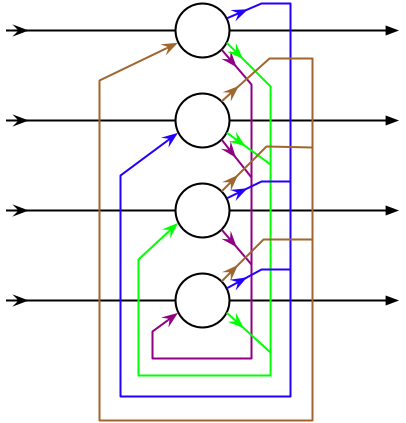
\includegraphics[width=10cm]{neuroinf_hopfieldnet.png}\\
Usage of Hopfield Network	& The Hopfield Network models \textbf{associative memory}. Given a initial state, the Hopfield Network converges to some stable state, which is similar to the initial state, whatever similar means. Memory by association (i.e. similarity) is a fundamentally different concept than memory by list lookup as it is done in computers.\\
Memory concepts		& \begin{tabular}[t]{lrcl}
			    Human:	& Initial input		& $\xrightarrow[]{Association}$	& Memorized information\\
			    Computer:	& Input index		& $\xrightarrow[]{List lookup}$	& Memorized information	
			  \end{tabular}\\
Nodes			& The nodes represent neurons, which can be modelled by McCulloch-Pitts Neurons, as an example. A neuron can either be active (1) or inactive (0, sometimes -1)\\
			& Let the activation state be denoted by $a_i$.\\
Edges			& An edge represent a connection between two neurons. The strength of an edge is modeled by its weight.\\
			& Let the weight of an edge be denoted by $w_{ij}$\\
Pattern			& The set of each node's state is called a pattern (i.e. 0000111110100).\\
Assumptions		& \begin{itemize}
           		  	\item No autoconnections.
				\item Weights between two neurons are the same (symmetric weights)
           		  \end{itemize}\\
Bias			& The bias is neglected. For computations, a extra neuron can be imposed which has a weight equal to the bias and which is always active.\\
Theorem			& A Hopfield network always converges to a stable configuration.\\
Energy			& $-\frac{1}{2} \sum_{i,j} w_{i,j} a_i a_j$ (if $a_i \in \{0,1\}$)\\
``Proof''		& We can define an algorithm according to which the energy must be minimized. That is, starting from an arbitrary initial condition, a neuron will be activated, if its weights contribute nonnegatively to the energy. This asynchronous update converges.\\
Update rule		& If the sum of all edges from activated nodes to the node to be updated is nonnegative, this node will be activated (value 1 is assigned). Otherwise it will be inactivated (valu 0 or -1). This update rule is applied to all nodes asynchronously (overall state can change from node to node) or synchronously (equal state for all nodes). For asynchronous updates, the update order influences the result.\\
Relation to Max-Flow-Min-Cut	& To minimize the energy, we want to ``remove'' edges with a very low (or even negative) weight. This can be done by finding the minimal cut of the Hopfield network and then inactivate all nodes on one side of the cut. The side with less nodes should be chosen.\\
Learning rules		& Learning a pattern means lowering its energy. In fact, a pattern to be remembered must be a local minimum. This can be achieved by adjusting the weights in such a way that the desired pattern has a minimal energy. One possible learning rule is Hebbian learning.\\
Hebbian learning	& \begin{tabular}[t]{l}
			    $w_{ij} = \frac{1}{N} \sum_{\mu=1}^p \epsilon_i^{\mu} \epsilon_j^{\mu}$
			    $N$: Number of neurons\\
			    $p$: Number of patterns to learn\\
			    $\epsilon_i^{\mu}$: State of bit $i$ of pattern $\mu$
			  \end{tabular}\\
Role of assumptions	& If the assumptions are broken, there are easy cases which lead to infinite cycling.\\
\end{longtable}
\section{Lecture 12: Feed-forward neural networks and Back-propagation}
\begin{tabular}{p{4cm}p{15cm}}
				& 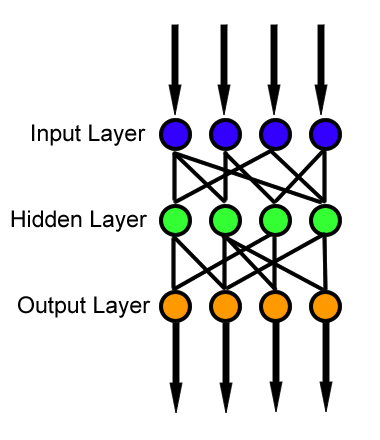
\includegraphics[width=10cm]{neuroinf_feedforward.png}\\
Feed-forward neural network	& In contrast to a recurrent neural network such as a Hopfield network, a FFNN, the connections between the neurons do not form a cycle. In a FFNN, information has only one direction: forward\\
Definitions		& \begin{tabular}[t]{l}
			    Let $N$ be the number of input signals\\
			    Let $D$ be the number of different input signals\\
			    Let $\vec{x}$ be the set of input signals (length $N$)\\
			    Let $\vec{f}$ be the set of network outputs (length $D$)\\
			    Let $\vec{g}$ be the set of desired network outputs (length $D$)
			  \end{tabular}\\
Error			& $E = \sum_i(f_i-g_i)^2$\\
Sigmoid function	& The output $f$ of an artificial neuron is given by $f = \mathrm{sgn} ( \mathbf{w^T x} + b)$, where $\mathbf{x}:$ inputs, $\mathbf{w}:$ weights, $b$: bias and assuming the boolean output is set as $f = \{-1,1\}$. Since the signum function is not continuous and not differentiable (?), we replace the signum function by the sigmoid function $f(y) = \frac{1}{1 + e^{-y}}$. The derivative of the sigmoid function is $\frac{df}{dy} = \frac{e^{-y}}{(1+e^{-y})^2} = y(1-y)$\\
Algorithm		& \begin{algorithmic}
			    \For {i = 0; i $<$ D; i++}
				\State Feed input $(\vec{x})_i$ to network. Compute $f_i - g_i$
				\For{each weight $w_k$}
				  \State Compute sensitivity of output: $\frac{df_i}{dw_k}$
				  \State $w_k = w_k-\epsilon (f_i-g_i) \frac{df_i}{dw_k}$ ($\epsilon$ is the learning rate)
				\EndFor
			    \EndFor
			  \end{algorithmic}\\
\end{tabular}